\documentclass{article}

\usepackage{graphicx}
\usepackage{tikz}
\usepackage{tikzsymbols}
\usetikzlibrary{calc,patterns,shapes.geometric}
\pagestyle{empty}
\usepackage[margin=0pt]{geometry}
\geometry{papersize={14in,12in}}

\def\centerarc[#1](#2)(#3:#4:#5){\draw[#1] ($(#2)+({#5*cos(#3)},{#5*sin(#3)})$) arc (#3:#4:#5);}

\begin{document}
	\begin{figure}
		\centering
		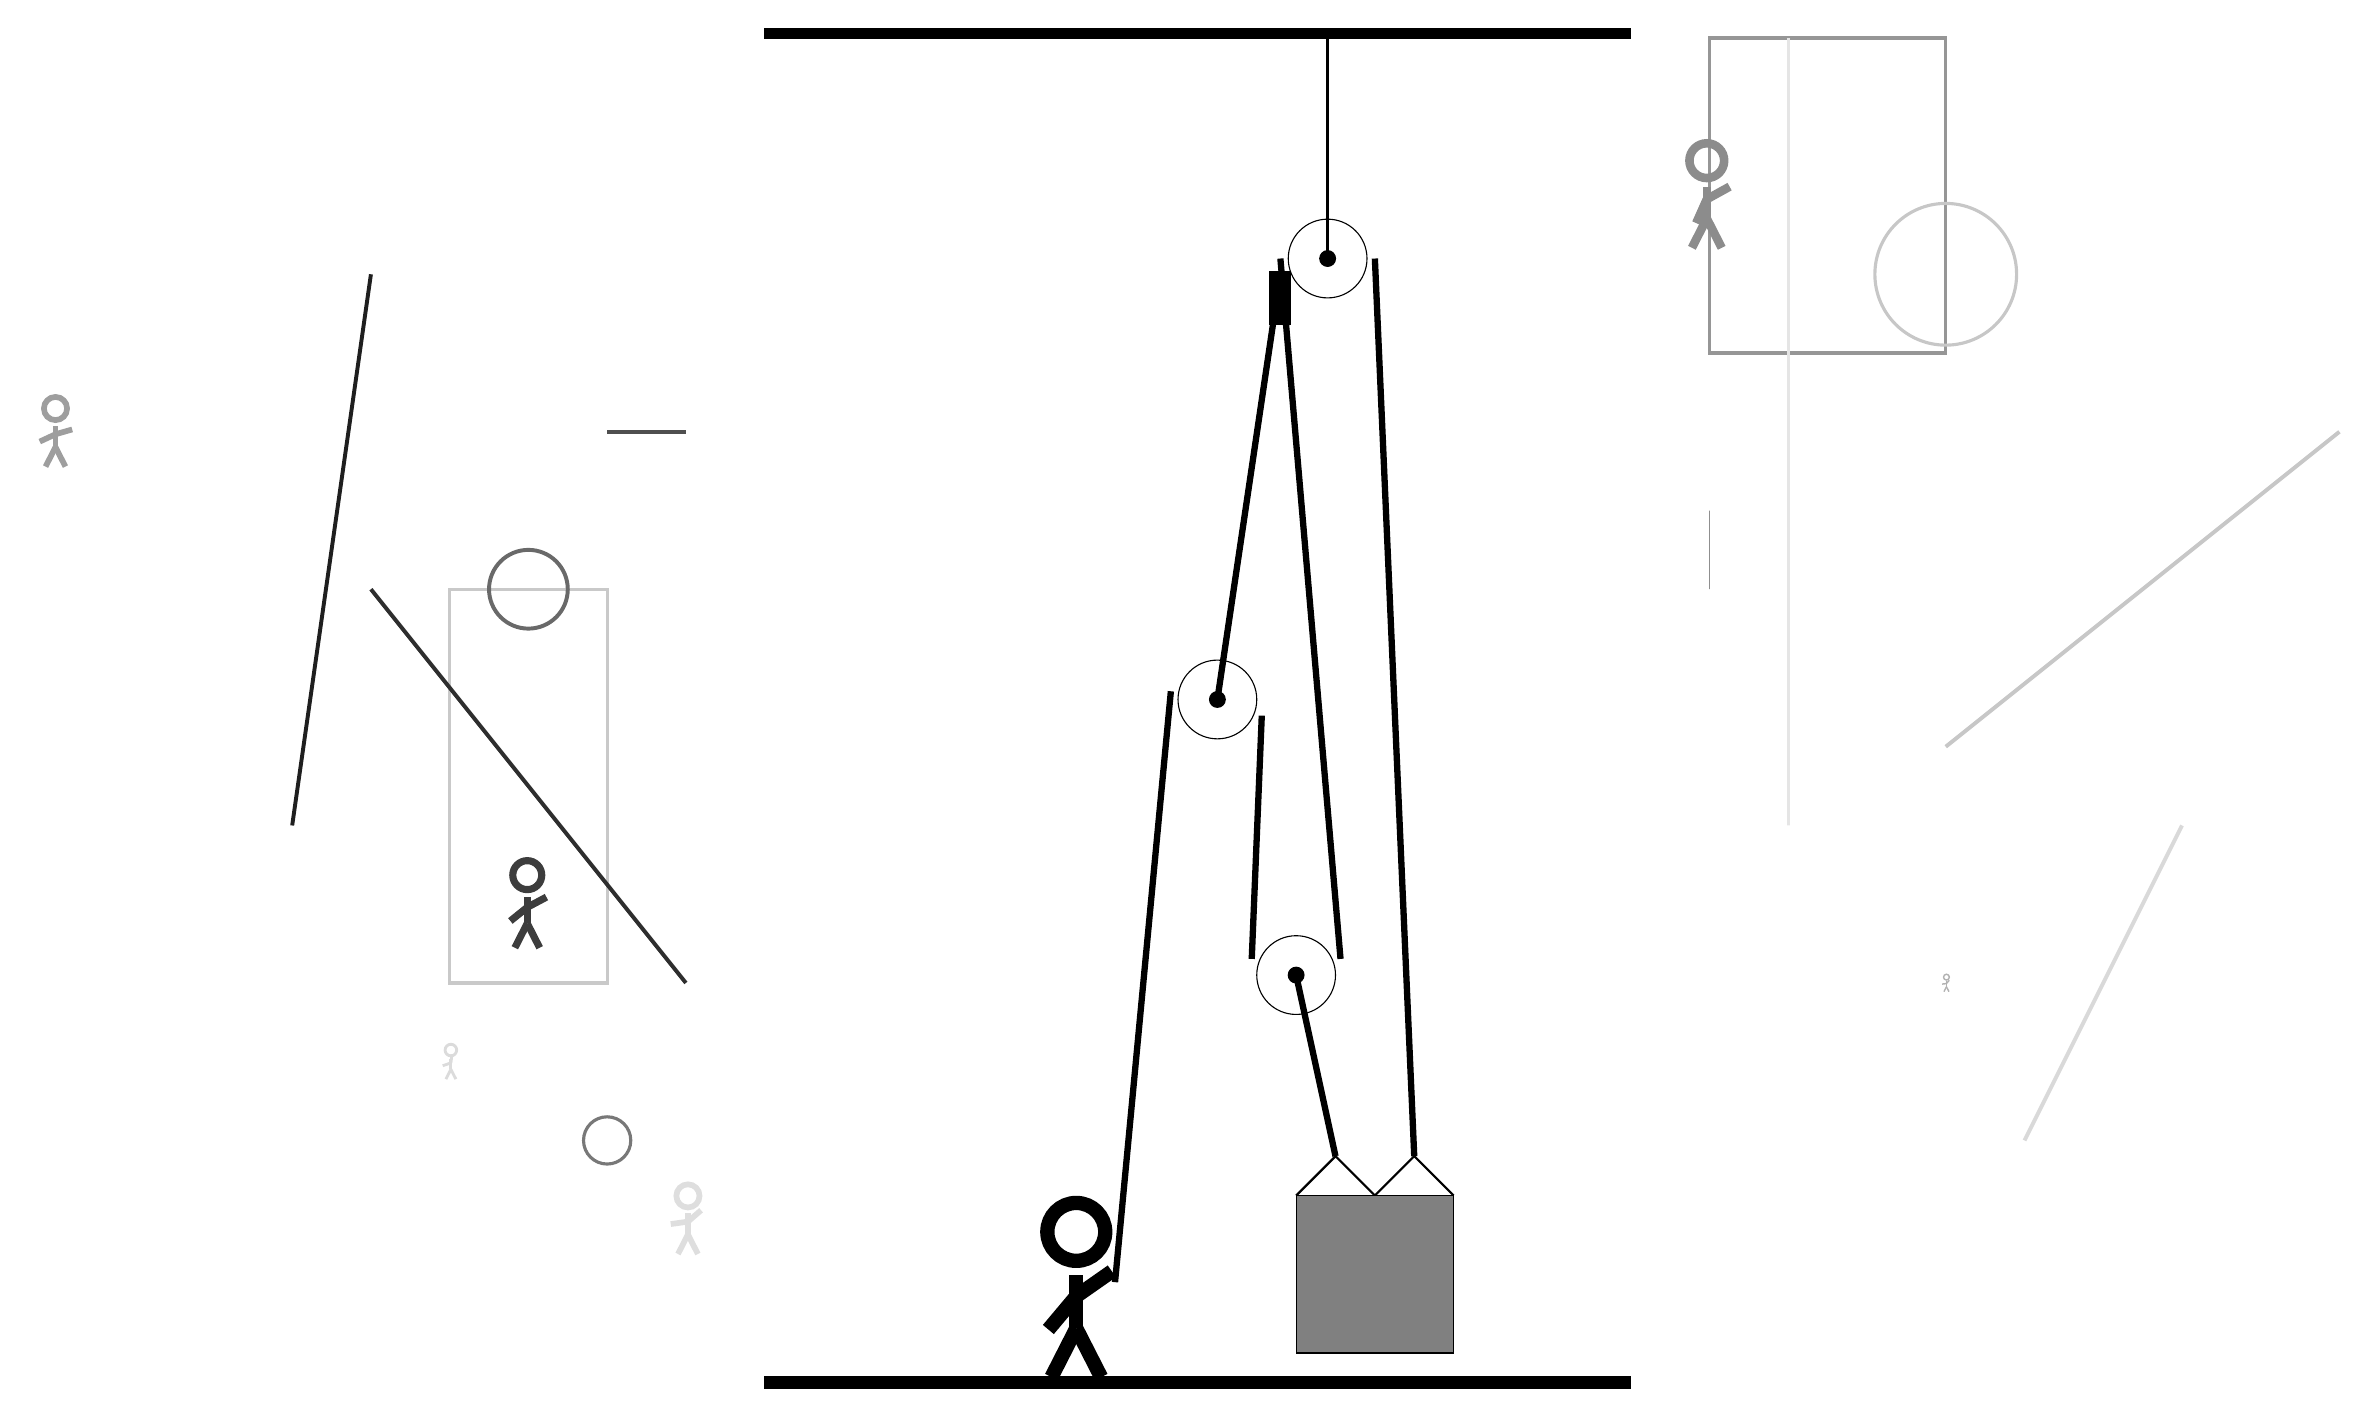
\begin{tikzpicture}
			%%%%% START %%%%%
			
			\draw[fill=black] (-6, 14) rectangle (5, 14.125);
			
			\draw (-0.25, 5.6) circle (0.5);
			\draw[fill=black] (-0.25, 5.6) circle (0.1);
			
			\draw (0.75, 2.1) circle (0.5);
			\draw[fill=black] (0.75, 2.1) circle (0.1);
			
			\draw (1.15, 11.2) circle (0.5);
			\draw[fill=black] (1.15, 11.2) circle (0.1);
			\draw[very thick] (1.15, 11.2) -- (1.15, 14);
			
			\node[line width=0.5mm, color=black!38] at (-15, 9) {\Strichmaxerl[4][25][16]};
			
			\draw[line width=0.4mm, color=black!21] (-8, 2) rectangle (-10, 7);
			\node[line width=0.7mm, color=black!30] at (9, 2) {\Strichmaxerl[1][7][50]};
			\draw[line width=0.5mm, color=black!88](-11, 11) -- (-12, 4);
			
			\draw [line width=0.4mm, color=black!53](-8, 0) circle (0.3);
			\node[line width=0.3mm, color=black!13] at (-7, -1) {\Strichmaxerl[4][8][41]};
			\draw[line width=0.2mm, color=black!44] (6, 8) rectangle (6, 7);
			\node[line width=0.6mm, color=black!14] at (-10, 1) {\Strichmaxerl[2][19][83]};
			\draw[line width=0.4mm, color=black!41] (6, 14) rectangle (9, 10);
			\draw[line width=0.4mm, color=black!10] (7, 4) rectangle (7, 14);
			\draw[line width=0.5mm, color=black!15](10, 0) -- (12, 4);
			\draw[line width=0.5mm, color=black!22](9, 5) -- (14, 9);
			\node[line width=0.5mm, color=black!76] at (-9, 3) {\Strichmaxerl[5][39][28]};
			
			\draw[line width=0.5mm, color=black!69] (-8, 9) rectangle (-7, 9);
			\draw [line width=0.5mm, color=black!59](-9, 7) circle (0.5);
			\node[line width=0.3mm, color=black!45] at (6, 12) {\Strichmaxerl[6][66][29]};
			
			\draw[line width=0.5mm, color=black!82](-7, 2) -- (-11, 7);
			
			\draw [line width=0.4mm, color=black!22](9, 11) circle (0.9);
			\draw[line width=0.6mm, color=black!27] (-8, 1) rectangle (-8, 1);
			\draw [line width=0.4mm, color=black!78](8, 6) circle (0.0);
			
			\draw[thick]  (0.75, -0.7) -- (1.25, -0.2) -- (1.75, -0.7) -- (2.25, -0.2) -- (2.75, -0.7);
			\draw[fill=black!50] (0.75, -0.7) rectangle (2.75, -2.7);
			
			\draw[line width=0.8mm] (-0.25, 5.6) -- (0.55, 11.0);
			\draw[line width=0.8mm, fill=black](0.45, 10.4) rectangle (0.65, 11.0);
			\draw[line width=0.8mm] (-1.55, -1.8) -- (-0.8409, 5.7042);
			\centerarc[line width=0.8mm](-0.25, 5.6)(-20:170:0.6);
			\draw[line width=0.8mm] (0.3138, 5.3948) -- (0.1862, 2.3052);
			\centerarc[line width=0.8mm](0.75, 2.1)(160:380:0.6);
			\draw[line width=0.8mm] (1.3138, 2.3052) -- (0.55, 11.2);
			\draw[line width=0.8mm](0.75, 2.1) -- (1.25, -0.2);
			\centerarc[line width=0.8mm](1.15, 11.2)(0:180:0.6);
			\draw[line width=0.8mm] (1.75, 11.2) -- (2.25, -0.2);
			
			\node at (-2, -1.9) {\Strichmaxerl[10][50][35]};
			
			\draw[fill=black] (-6, -3) rectangle (5, -3.15);
			
			%%%%% END %%%%%
		\end{tikzpicture}
	\end{figure}	
\end{document}